\section{Frequency mode 17}
\label{FM17}

\subsection{Spectra}
\label{FM17:spectra}

\begin{figure}[ht]
    \centering
    \begin{subfigure}[b]{0.9545\textwidth}
        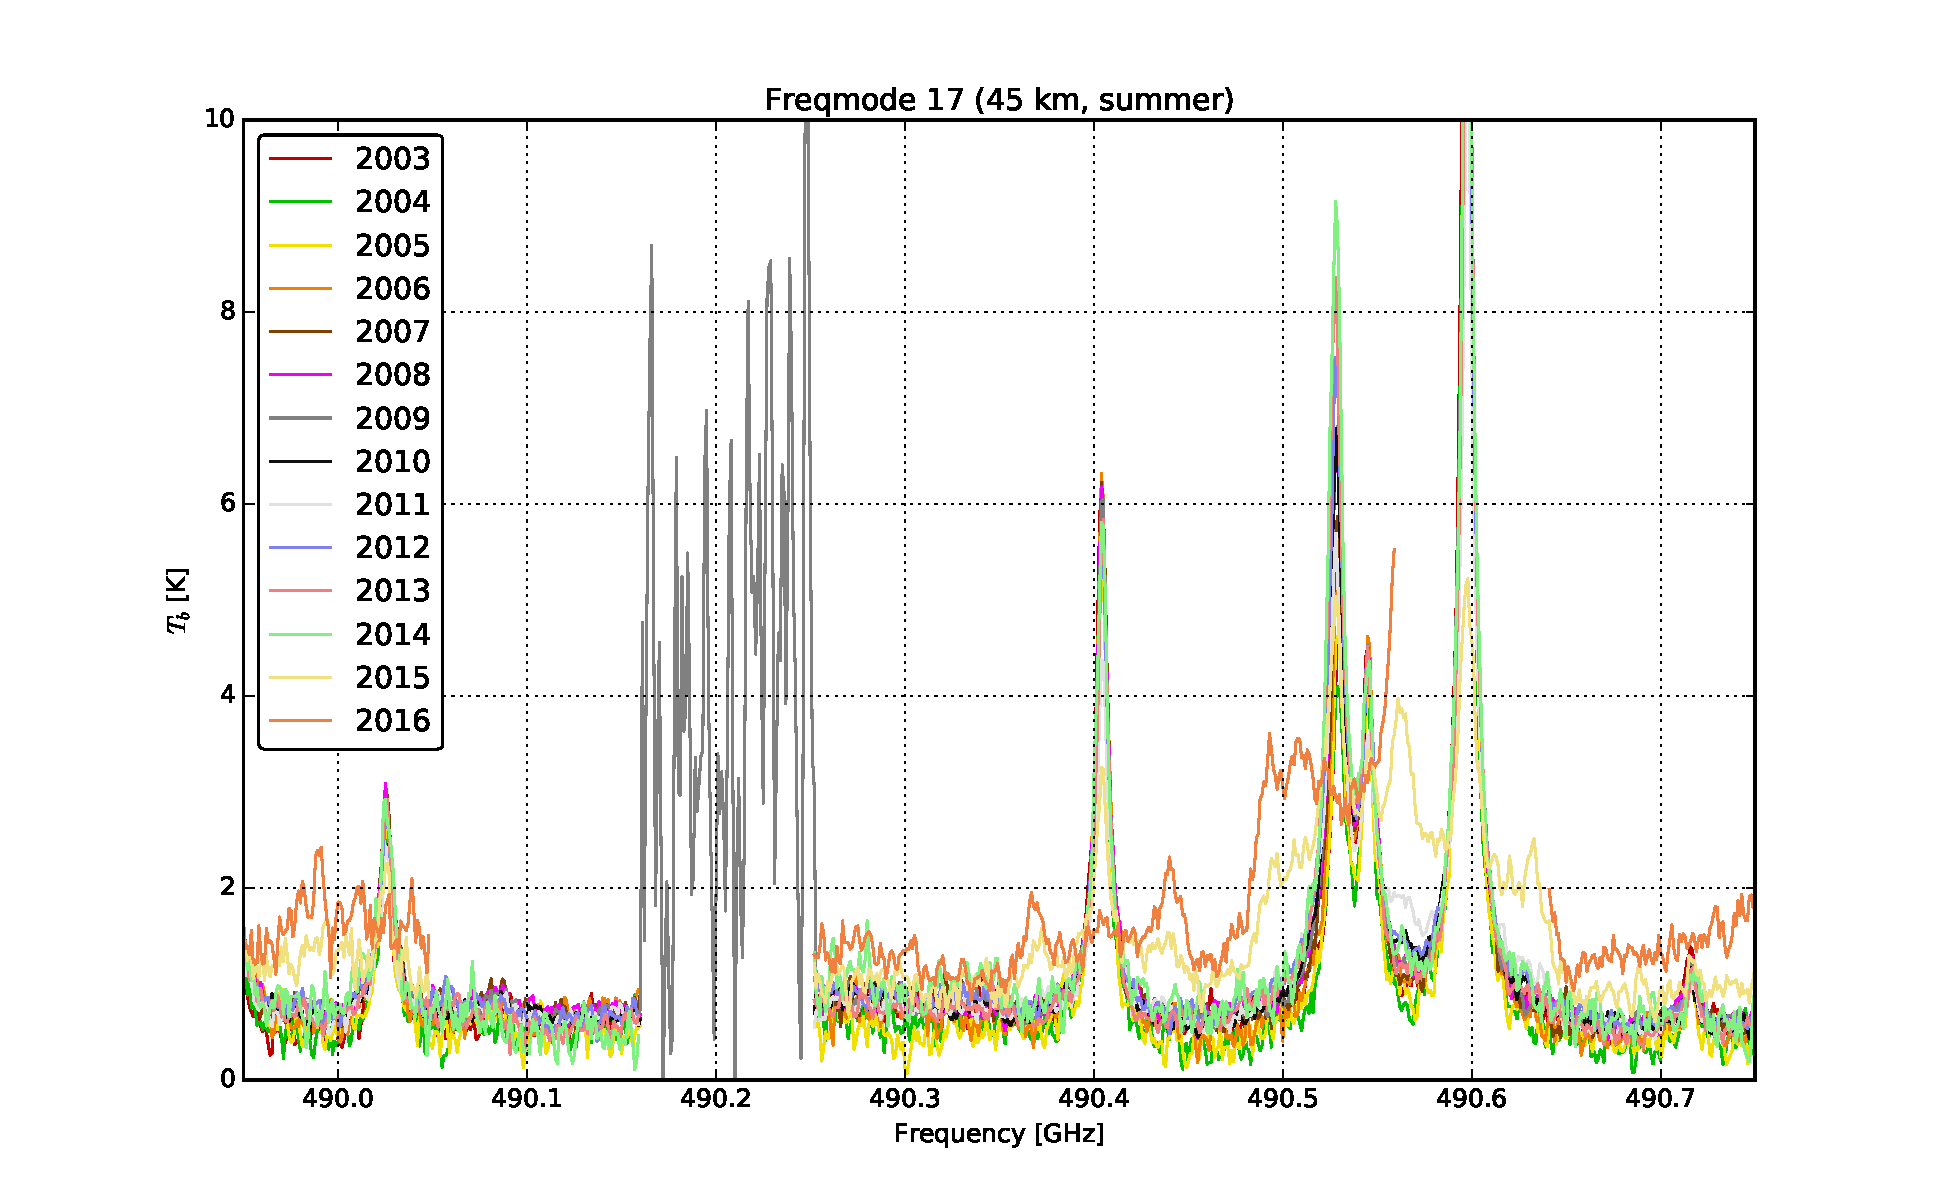
\includegraphics[width=\textwidth]{spectra/fm_17_spectra_summer}
        \caption{summer}\label{fig:spectra:17:summer}
    \end{subfigure}
    \begin{subfigure}[b]{0.9545\textwidth}
        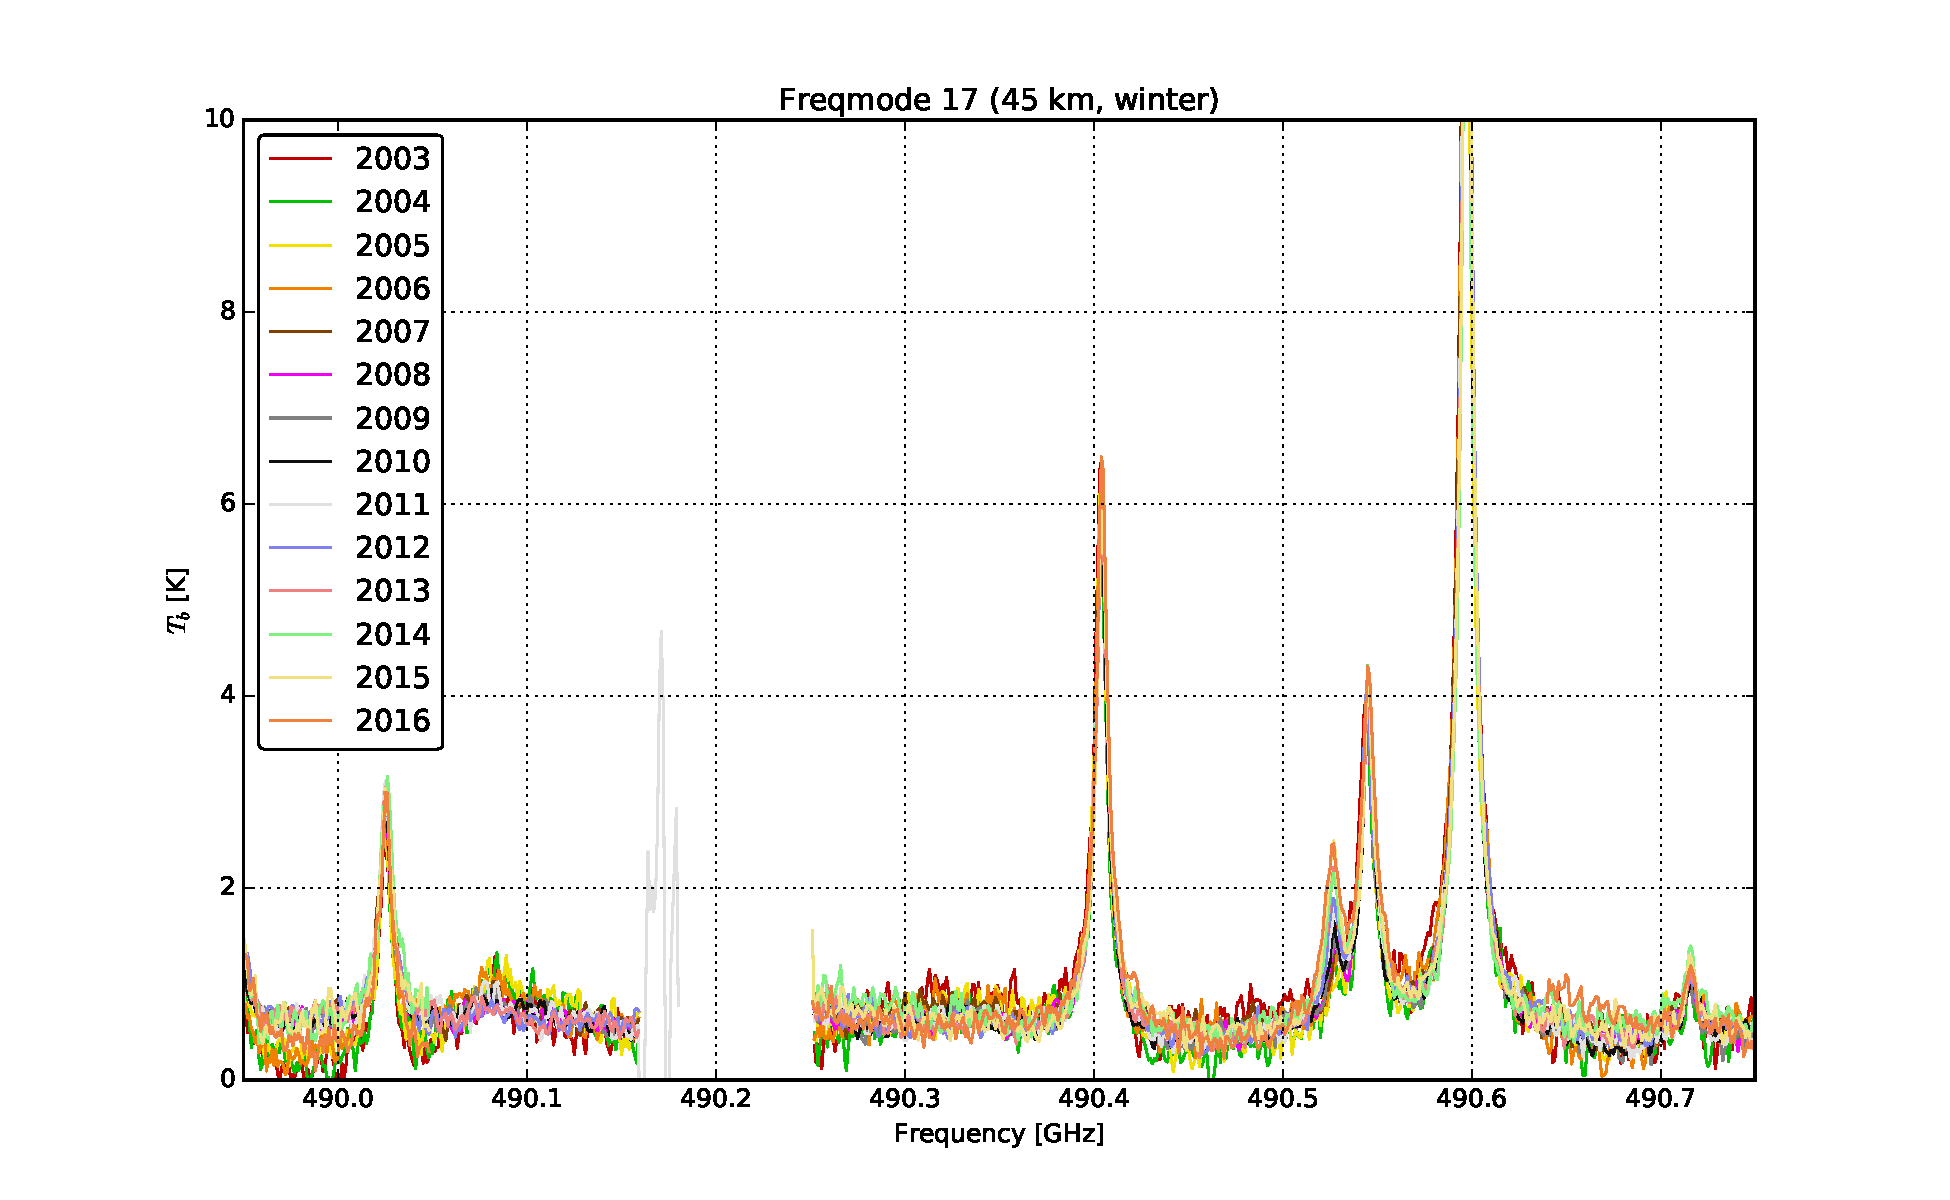
\includegraphics[width=\textwidth]{spectra/fm_17_spectra_winter}
        \caption{winter}\label{fig:spectra:17:winter}
    \end{subfigure}
    \caption{Annual median spectra for FM~17 for altitude interval 40--45~km
        at equatorial latitudes.  The main band peaks are \chem{O^{18}OO}
        at~$\sim490.03\,\mathrm{GHz}$, \chem{OO^{18}O}
        at~$\sim490.40$ and~$490.54\,\mathrm{GHz}$, \chem{HDO}
        at~$\sim490.60\,\mathrm{GHz}$, and \chem{OO^{17}O}
        at~$\sim490.72\,\mathrm{GHz}$.  There is a an \chem{O^3} sideband peak
        from~$\sim497.97\,\mathrm{GHz}$ at~$\sim490.53\,\mathrm{GHz}$, just
        below the second \chem{OO^{18}O} peak.  The unhealthy sub-bands~7 and~3
        encompass the area bewteen~$\sim490.05$ and~$490.25\,\mathrm{GHz}$.
        }\label{fig:spectra:17}
\end{figure}

\begin{figure}[ht]
    \centering
    \begin{subfigure}[b]{0.9545\textwidth}
        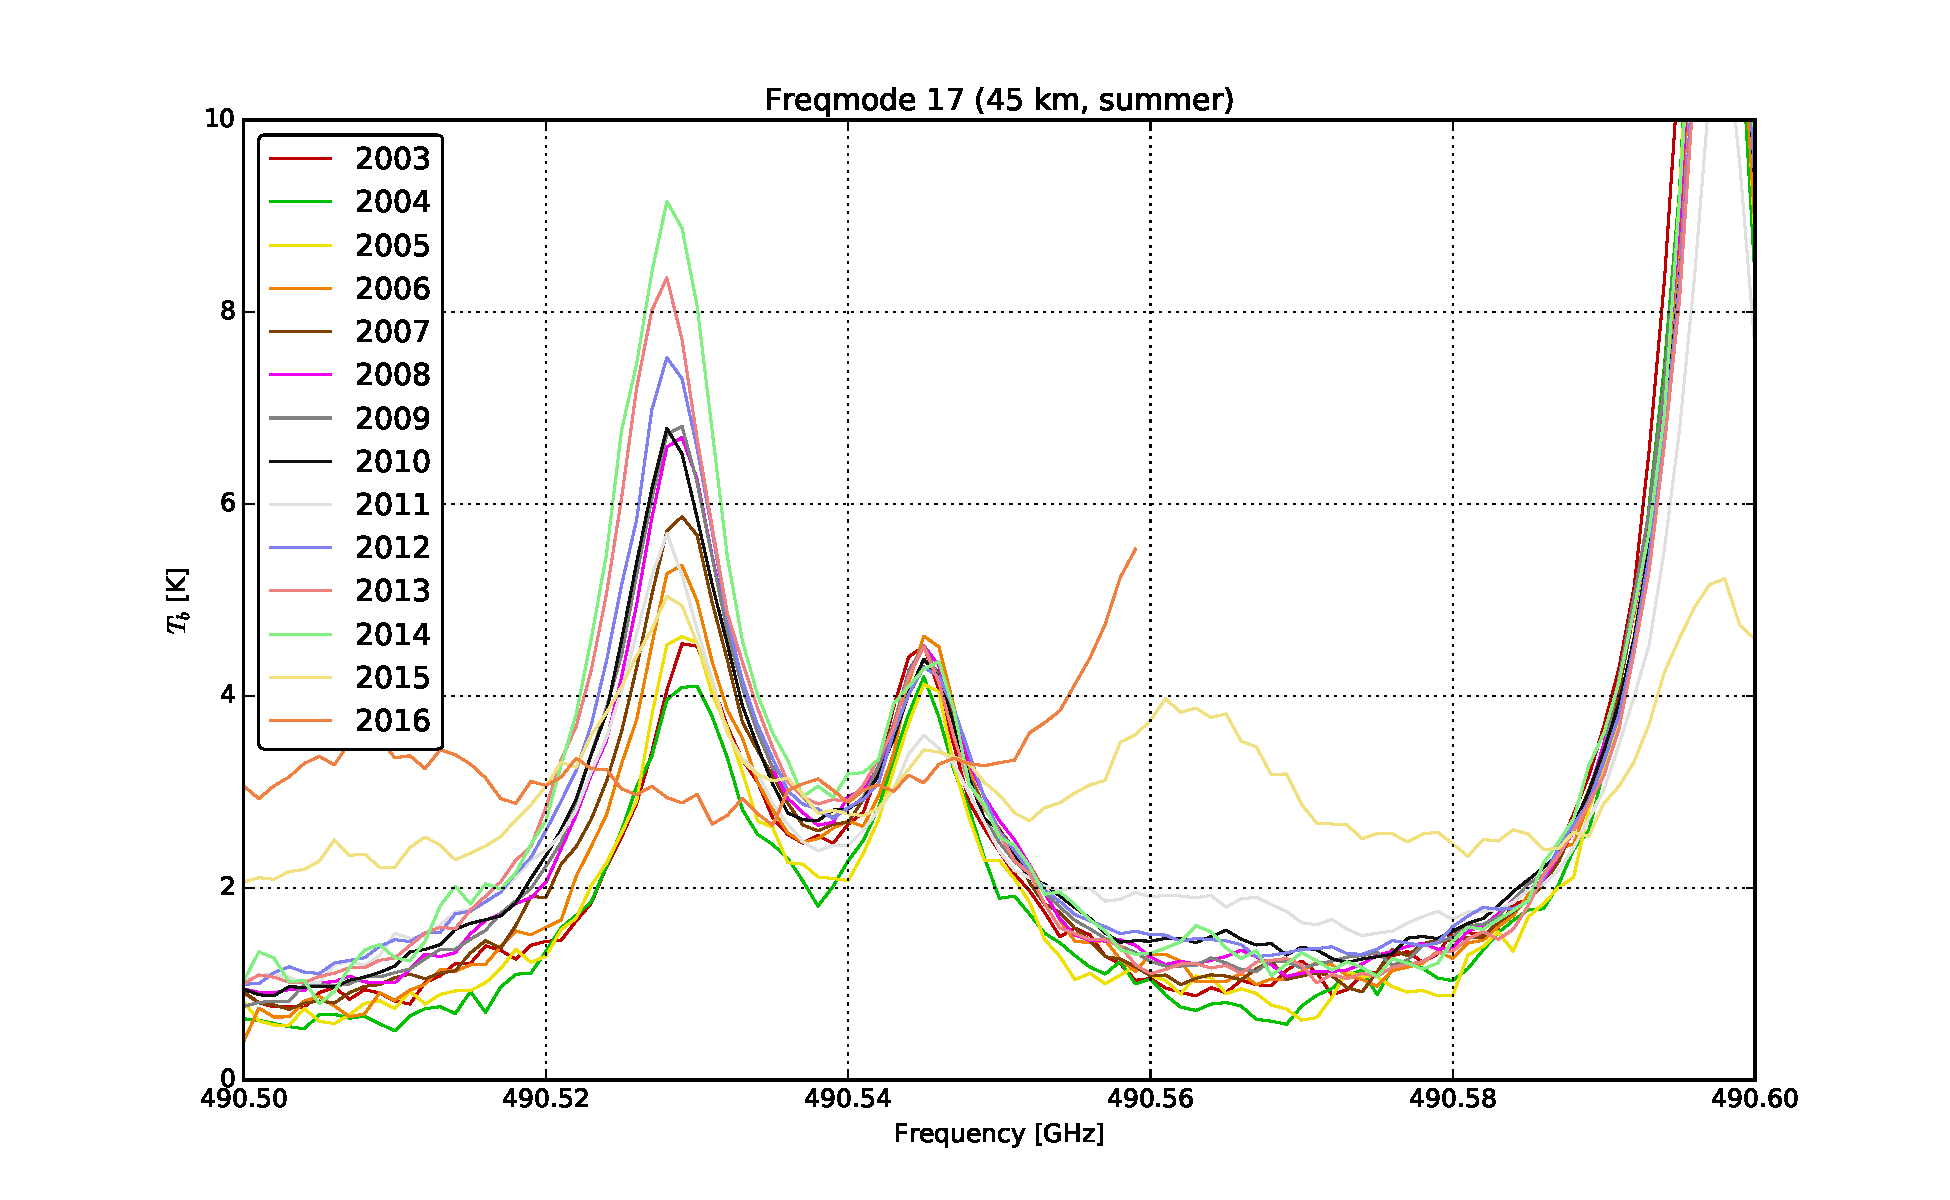
\includegraphics[width=\textwidth]{spectra/fm_17_spectra_summer_zoom}
        \caption{summer}\label{fig:spectra:17:summer:closeup}
    \end{subfigure}
    \begin{subfigure}[b]{0.9545\textwidth}
        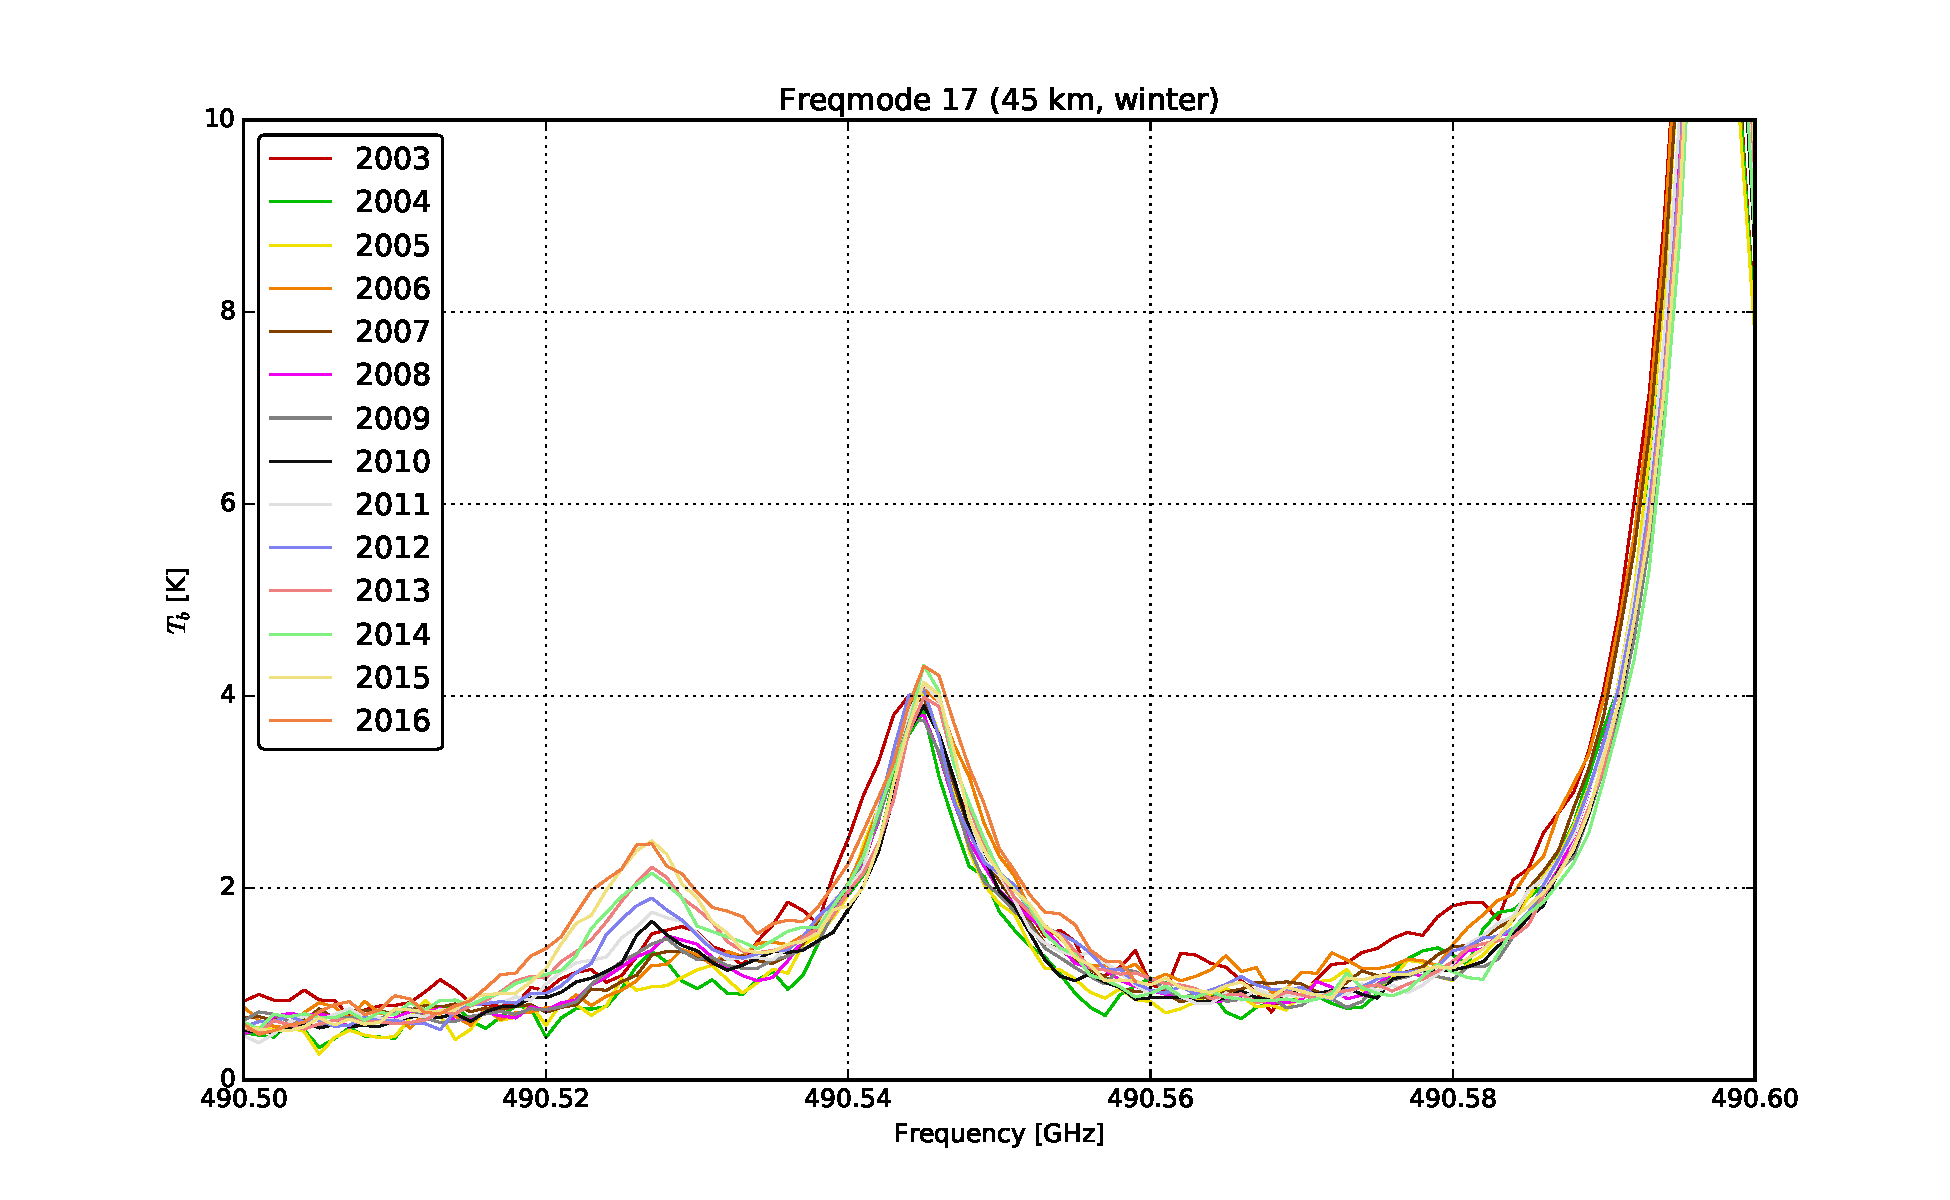
\includegraphics[width=\textwidth]{spectra/fm_17_spectra_winter_zoom}
        \caption{winter}\label{fig:spectra:17:winter:closeup}
    \end{subfigure}
    \caption{Close-up of Fig.~\ref{fig:spectra:17}, showing the \chem{OO^{18}O}
        peak at~$490.54\,\mathrm{GHz}$ and its neighbouring \chem{O^3} sideband
        peak from $\sim497.97\,\mathrm{GHz}$ at~$\sim490.53\,\mathrm{GHz}$.
        }\label{fig:spectra:17:closeup}
\end{figure}

\noindent
Yearly median spectra for summer and winter at $\sim45\,\mathrm{km}$ are shown
in Fig.~\ref{fig:spectra:17}.  These and the close-ups seen in
Fig.~\ref{fig:spectra:17:closeup} show that the spectra on the whole look sound,
except for in the summers of 2015 and 2016, when wing effects can be seen,
similar to those observed for FM~01.  It is also evident, in particular from
the close-ups, that the sideband leakage is higher during the summer, and that
it has been increasing over time.  Both of these observations are discussed in
more detail below.


\subsection{Wings}
\label{FM17:wings}
As can be seen in Fig.~\ref{fig:spectra:17:summer}, the median spectra from the
summers of 2015 and 2016 show markedly decreased main band peak amplitudes
coupled with the appearance of ghost peaks or ``wings'' approximately
$30\,\mathrm{MHz}$ to either side.  This is particularily evident for the
\chem{OO^{18}O} peak at~$\sim490.4\mathrm{GHz}$.  This is reminiscent of the
phenomenon afflicting FM~01, as discussed in Sec.~\ref{FM01:leftwings}.  For
FM~17, however, the effect is more clearly symmetric, more clearly peaked, and
furthermore occurs only during the summers, as opposed to during the winter,
which was the case for FM~01.  Though the idea of a common root cause is
enticing, these discrepancies, along with the fact that the problem only occurs
for 2015 and 2016 for FM~17, casts doubts on the hypothesis.  The problem could
also be explained by an unstable frequency correction, shifting whole
individual spectra up or down by a few tens of $\mathrm{MHz}$, something which
has all but been ruled out as the cause for the wings observed in the FM~01
spectra.  Further investigation, e.g.~by looking at time series of individual
spectra, would be necessary before drawing any firm conclusions.


\subsection{Sideband leakage}
\label{FM17:sbl}

\begin{figure}[ht]
    \centering
    \begin{subfigure}[b]{0.9545\textwidth}
        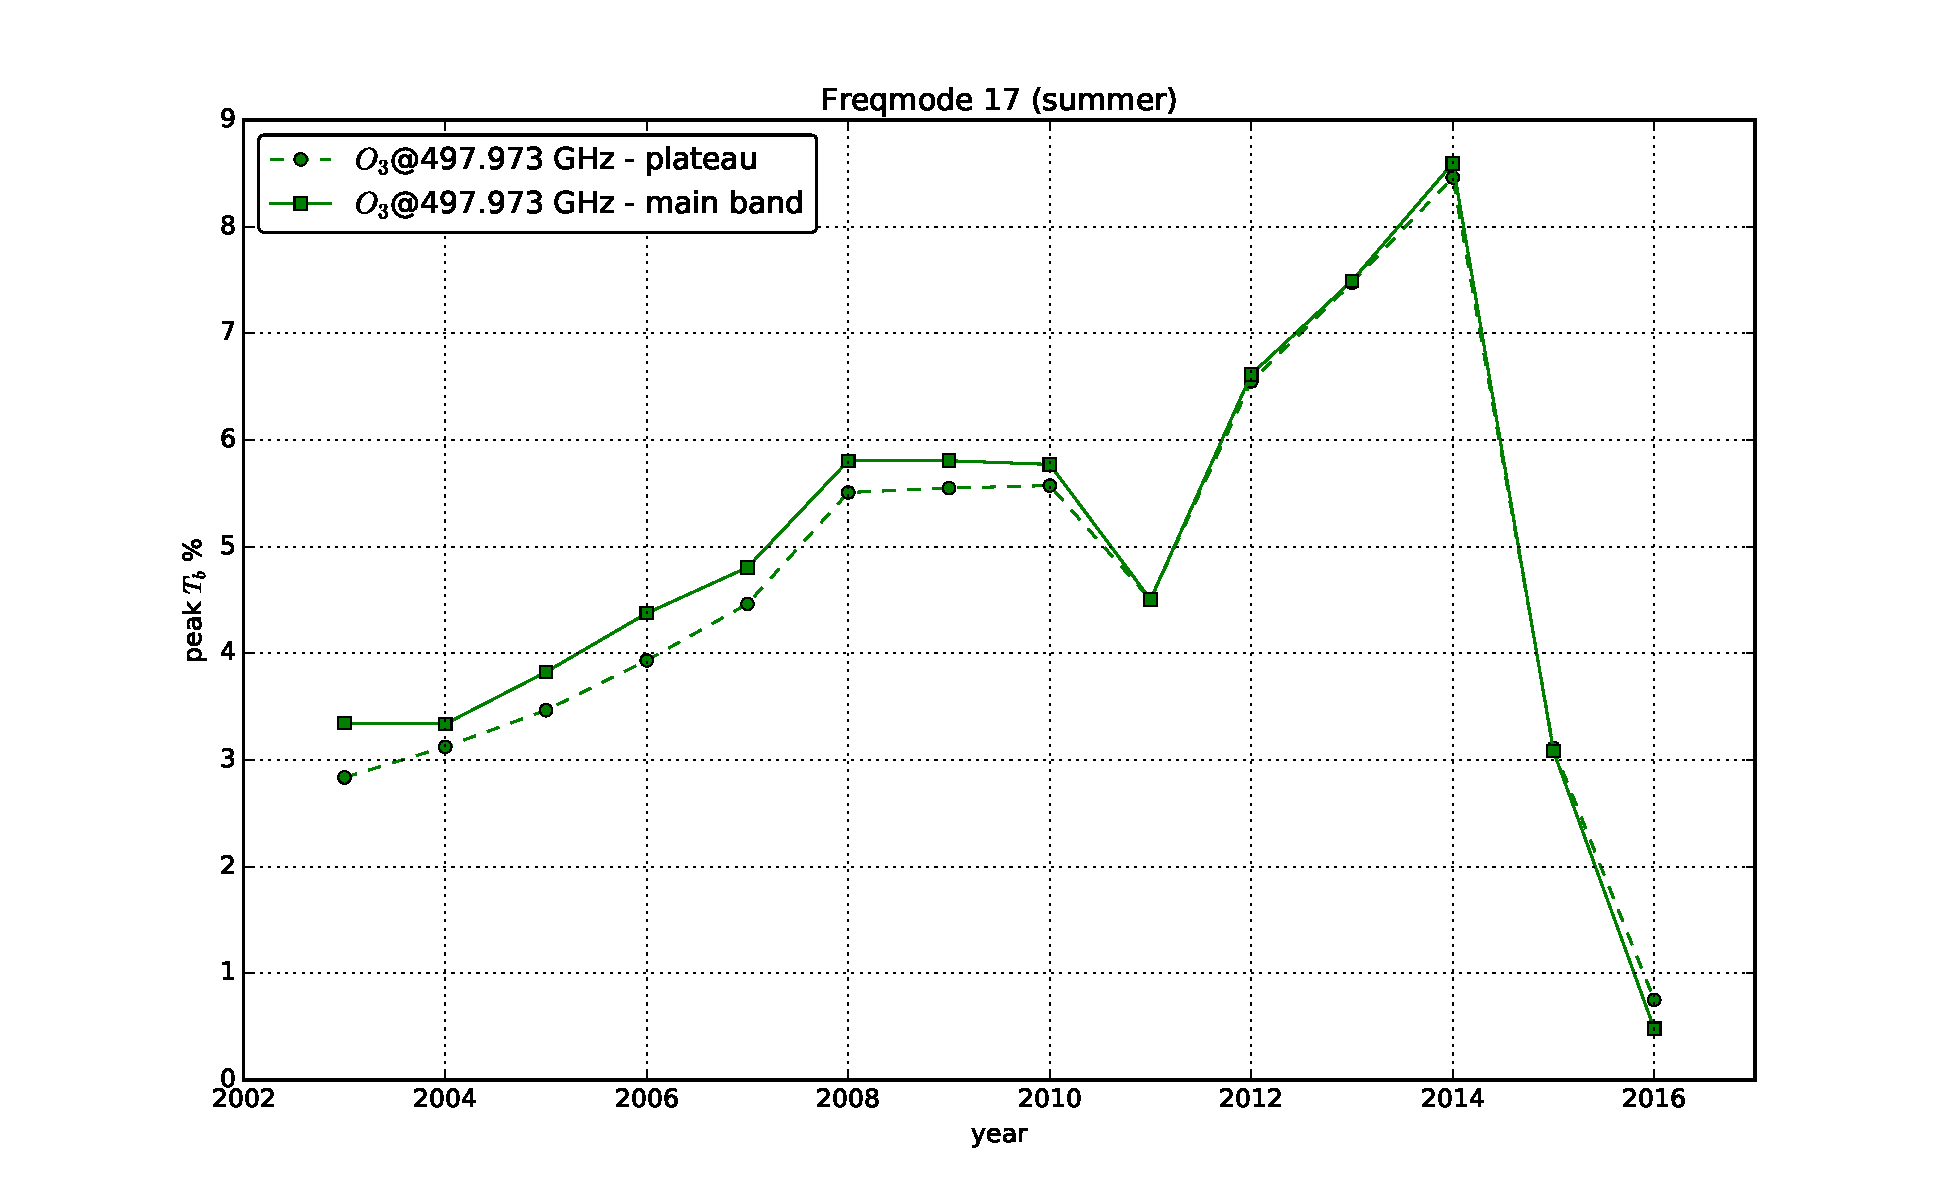
\includegraphics[width=\textwidth]{peaks/fm_17_sbl_summer}
        \caption{summer}\label{fig:sbl:17:summer}
    \end{subfigure}
    \begin{subfigure}[b]{0.9545\textwidth}
        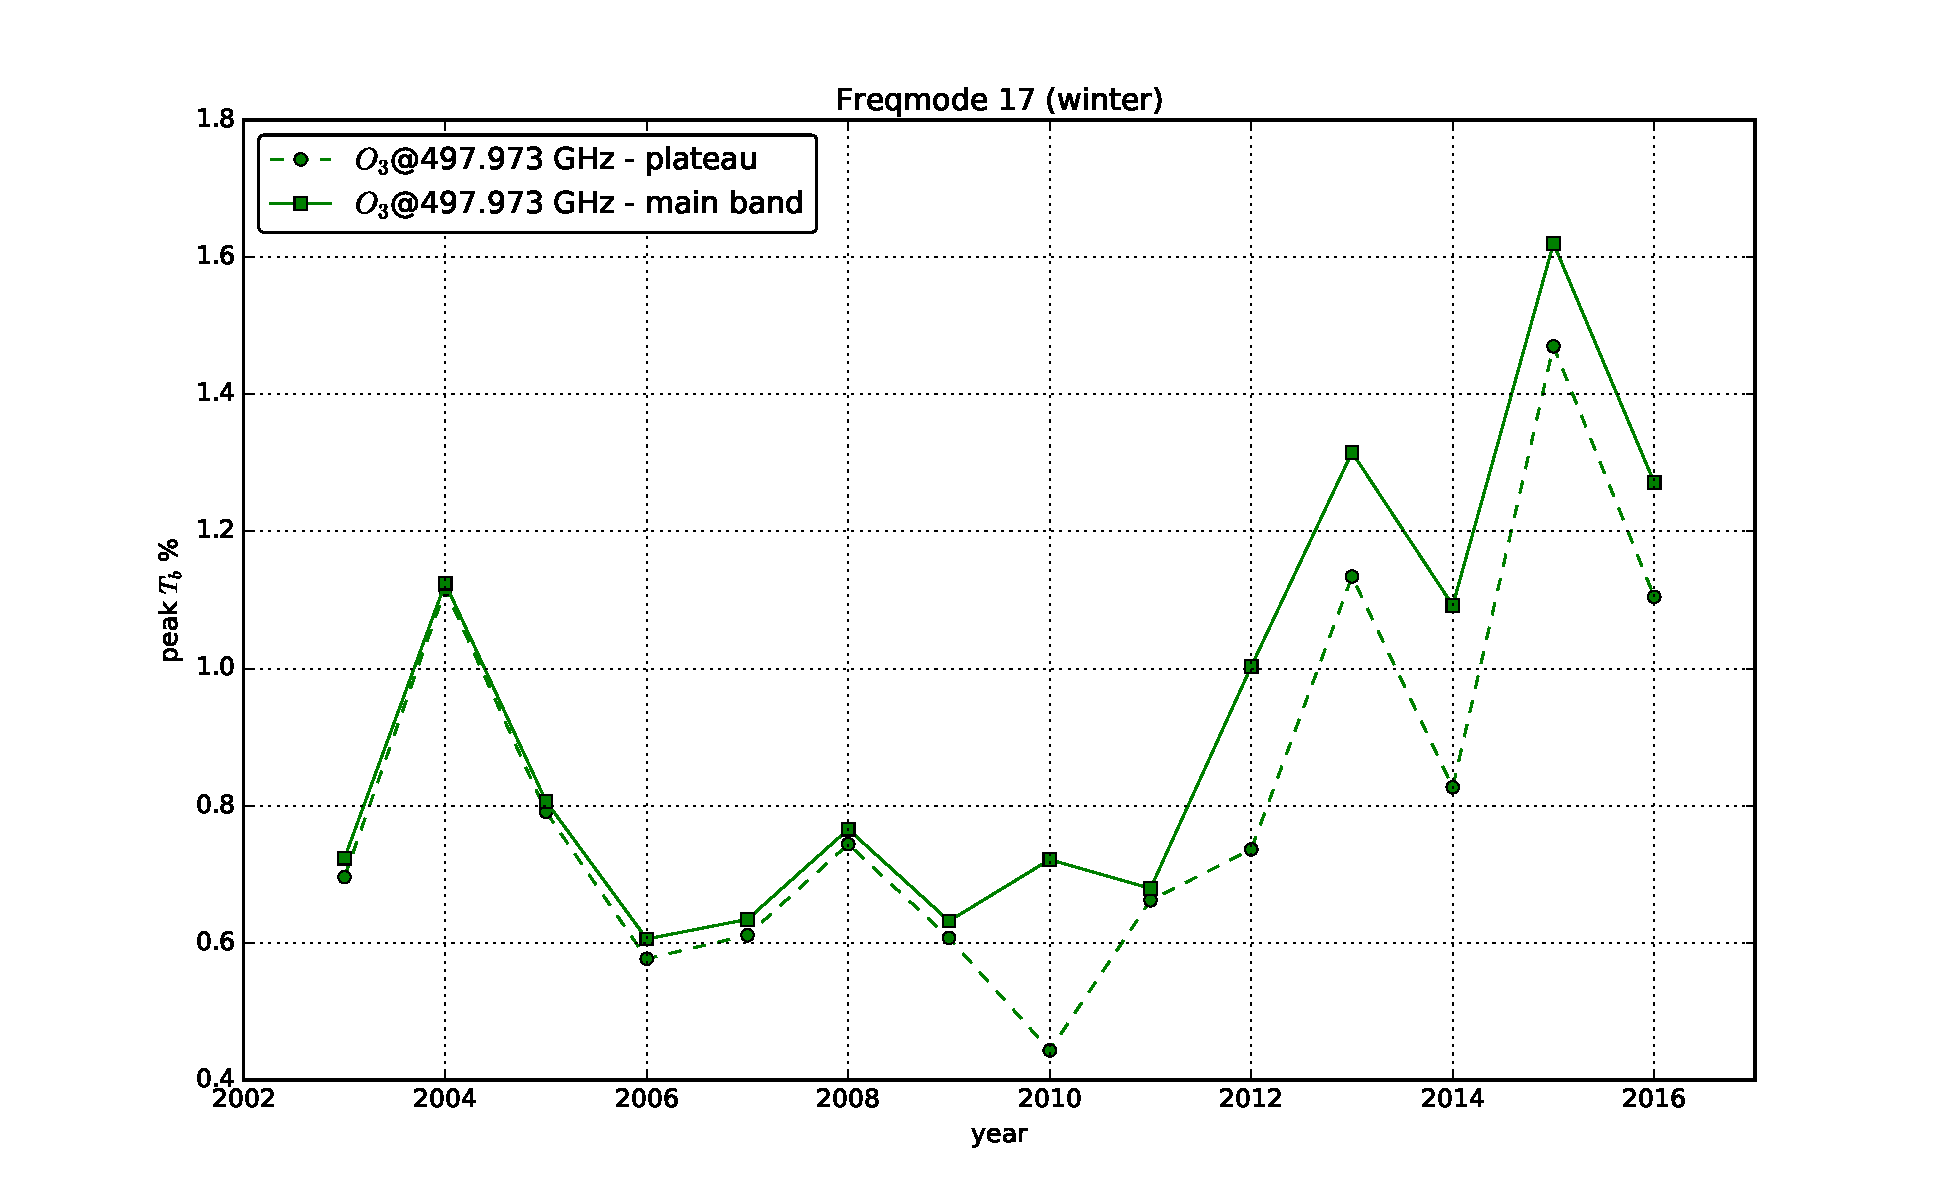
\includegraphics[width=\textwidth]{peaks/fm_17_sbl_winter}
        \caption{winter}\label{fig:sbl:17:winter}
    \end{subfigure}
    \caption{Sideband leakages in \% calculated from the data shown in
        Fig.~\ref{fig:spectra:17:closeup}. Values were calculated by
        subtracting the value of the ``plateau'' on the side the peak nearest
        its neighbouring main band peak, or a first order approximation of the
        main band value under the peak.  The results were compared with
        $73.3\,\mathrm{K}$, a value deemed representative of the actual peak
        intensity.}\label{fig:sbl:17}
\end{figure}

\noindent
The sideband leakage was estimated at $\sim45\,\mathrm{km}$ by taking the
sideband peak intensities from the data shown in
Figs.~\ref{fig:spectra:17:closeup} and subtracting the main band intensities
estimated by two methods:  by taking the value of the ``plateau'' on the side
of the peak nearest its neighbouring main band peak as the main band
value, and by making first order approximation of the value directly under the
peak.  The actual value should between these two estimates, but closer to the
latter.

To estimate the leakage, the extracted peak intensities were then divided by an
expected sideband peak intensity from simulations using
ARTS~(\cite{buehler:artst:05}).  $73.3\,\mathrm{K}$ was chosen as a
representative value for the sideband peak, but the peak value varies by
$\sim1\,\mathrm{K}$ from year to year.  The results are shown in
Figs.~\ref{fig:sbl:17}  where it can be seen that the sideband leakage during
the summer has been rising over time, from $\sim3\%$ to a remarkably high value
of almost $\sim9\%$ in 2014, after which the spectra for the summer became
unreliable (see~Fig.~\ref{fig:spectra:17:summer}).  During the winters, on the
other hand, the sideband leakage has fluctuated around $\sim1\%$, but shows a
increasing tendancy after 2010 up to $\sim1.5\%$.


\subsection{Seasonality}
\label{FM17:seasonailty}

\begin{figure}[ht]
    \centering
    \begin{subfigure}[b]{0.9545\textwidth}
        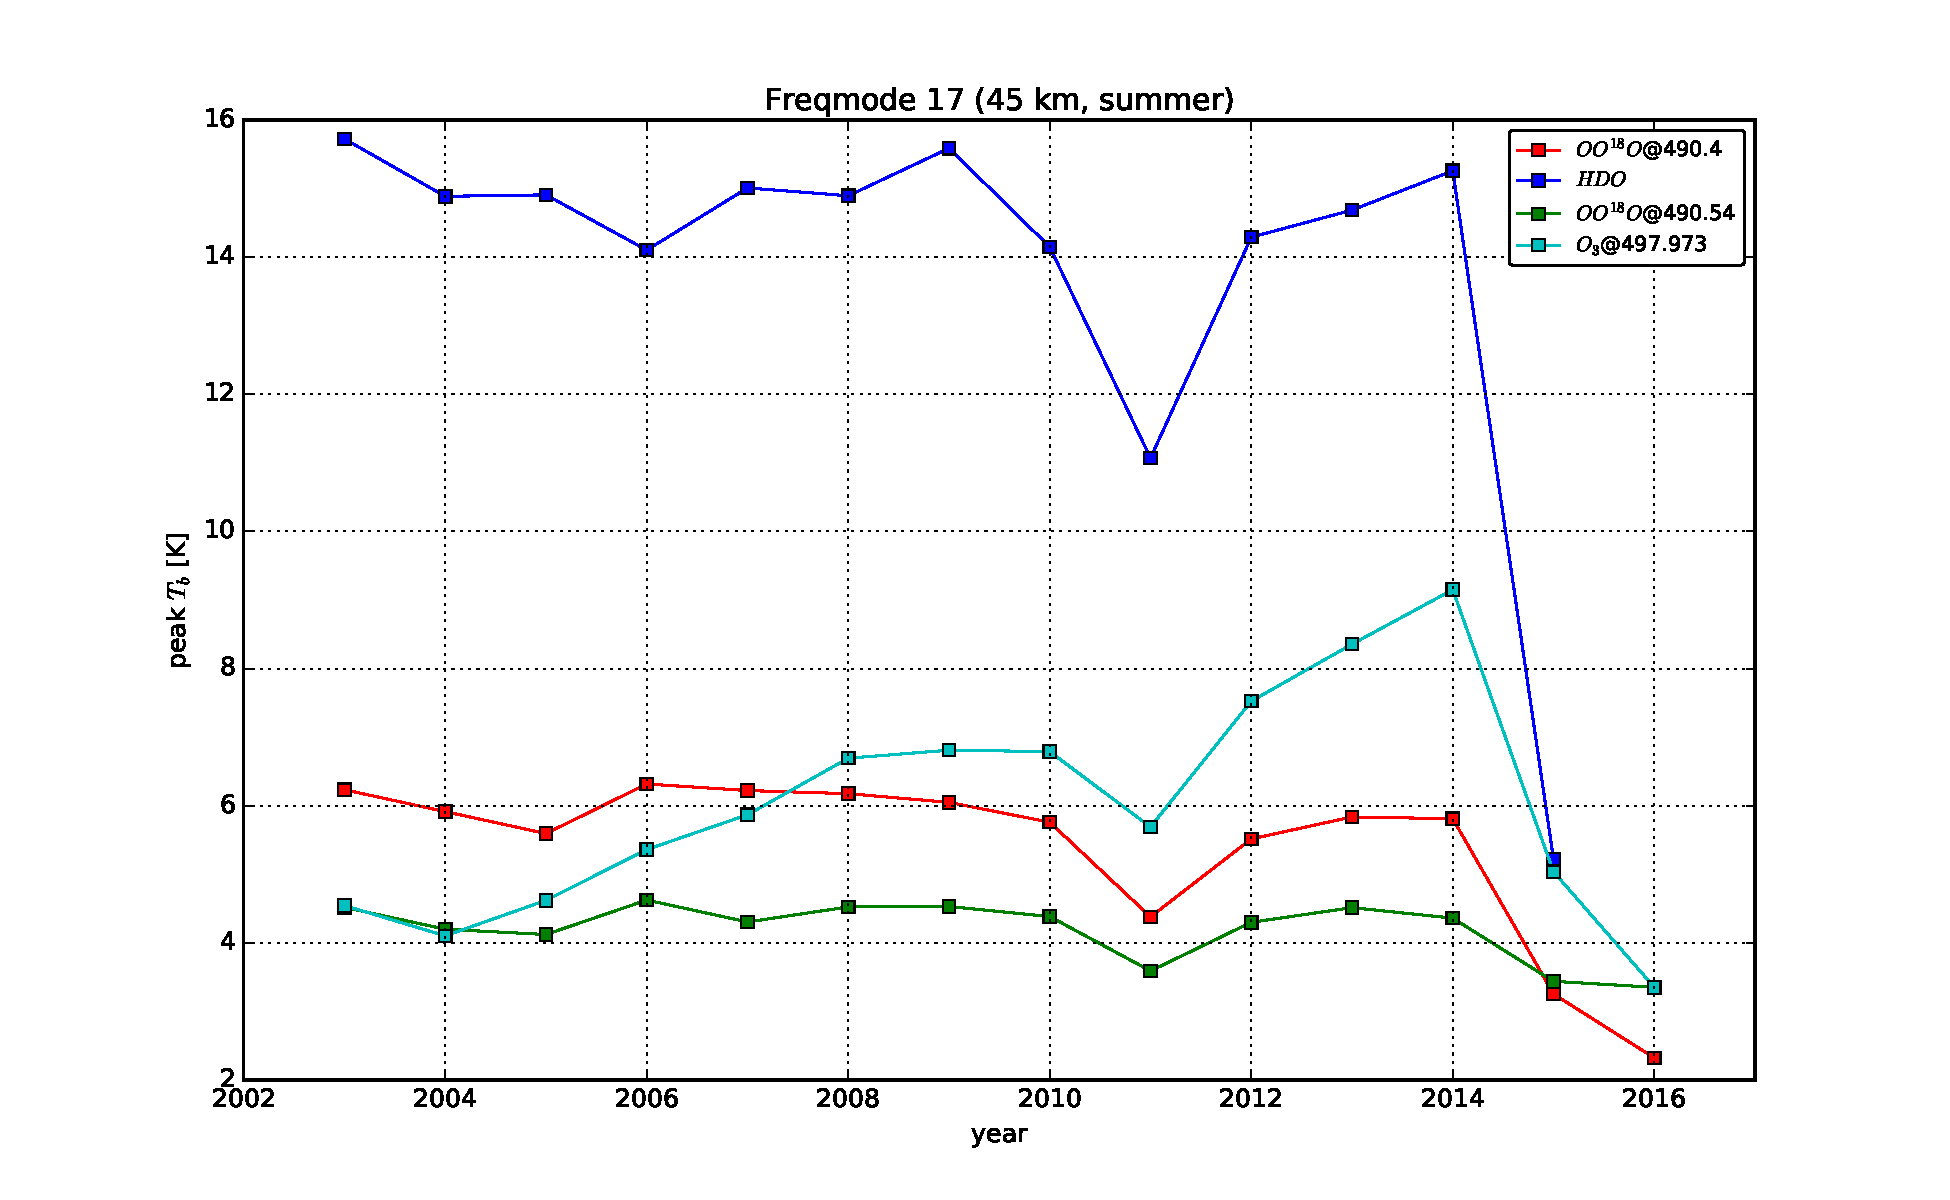
\includegraphics[width=\textwidth]{peaks/fm_17_peaks_summer}
        \caption{summer}\label{fig:peaks:17:summer}
    \end{subfigure}
    \begin{subfigure}[b]{0.9545\textwidth}
        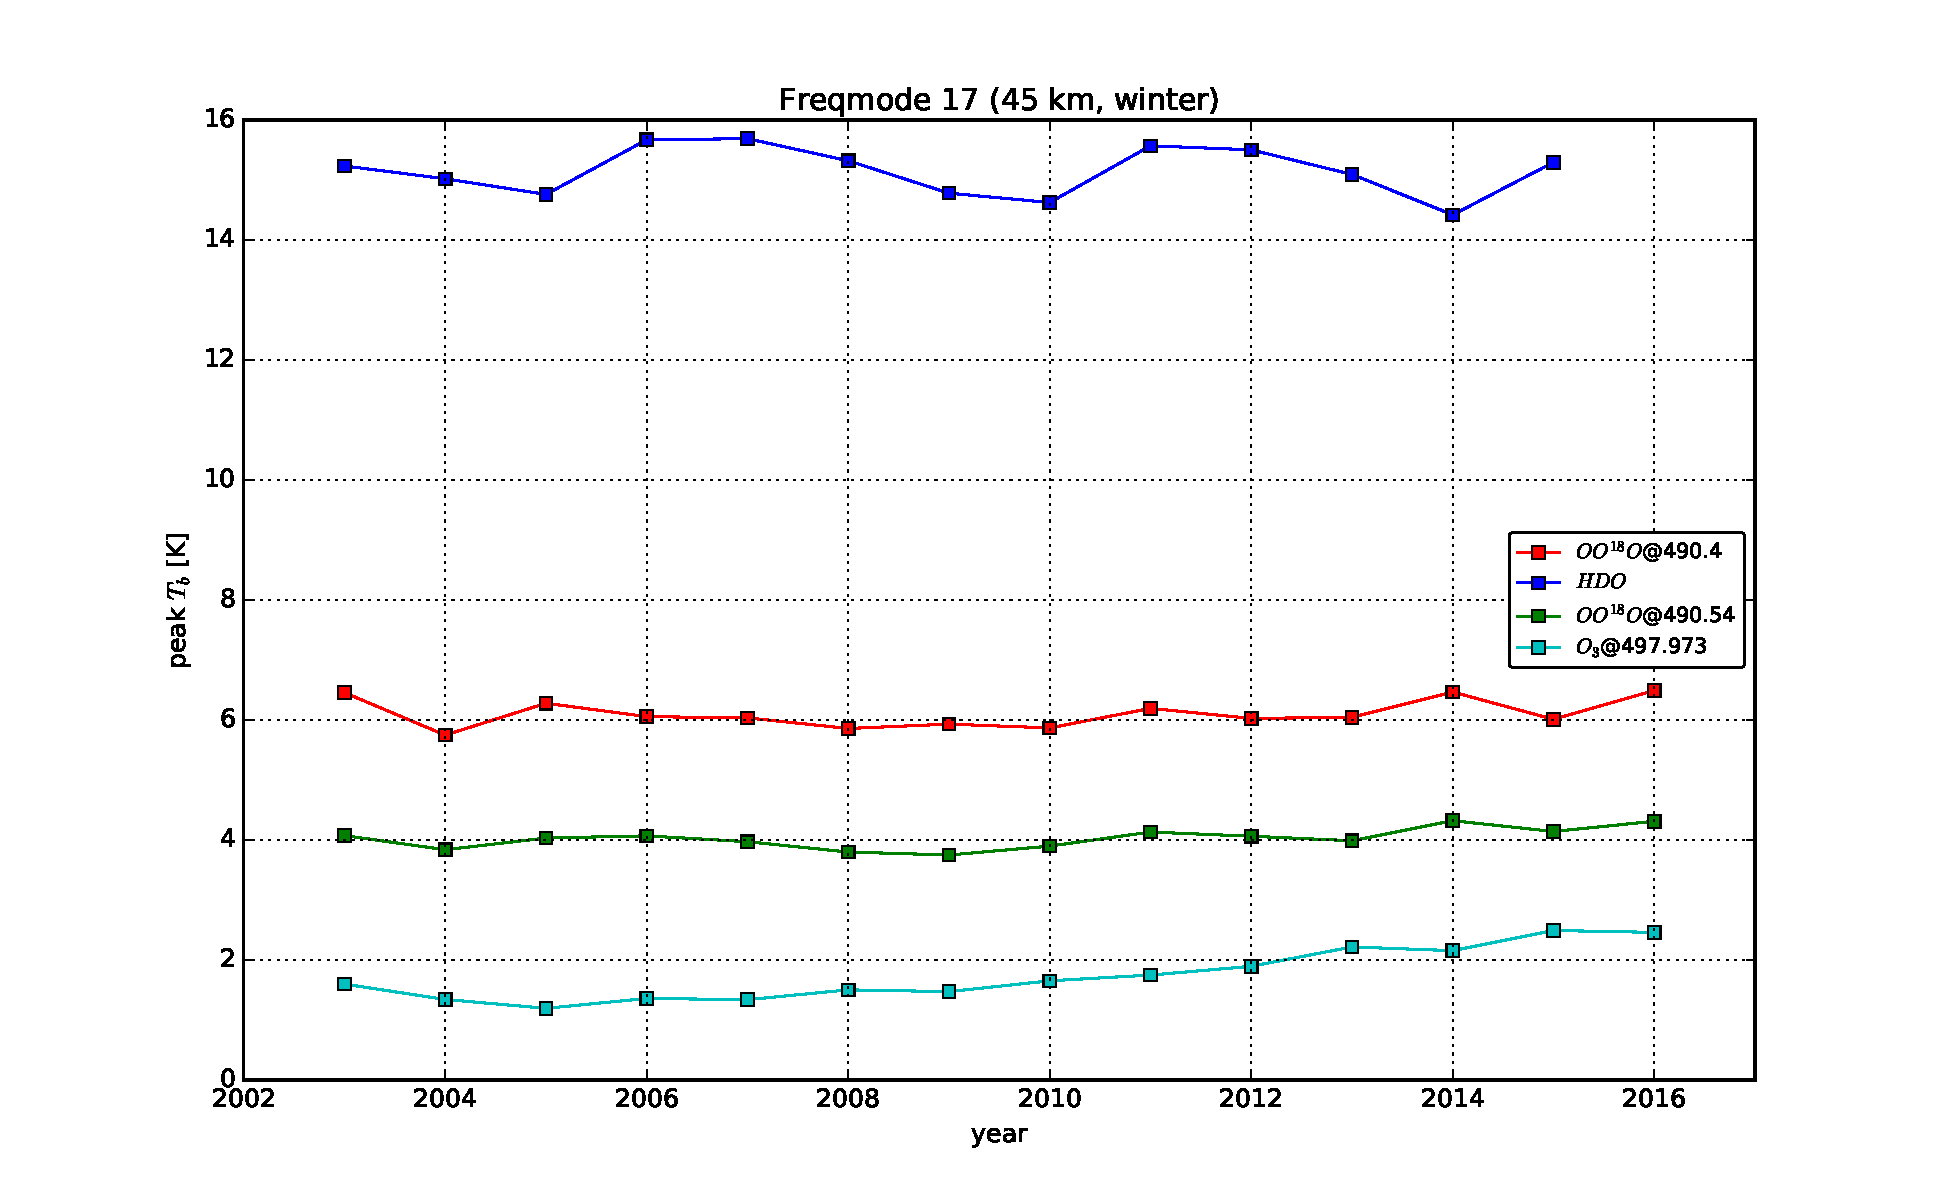
\includegraphics[width=\textwidth]{peaks/fm_17_peaks_winter}
        \caption{winter}\label{fig:peaks:17:winter}
    \end{subfigure}
    \caption{Annual median peak values for FM~17 for altitude interval
        40--45~km at equatorial latitudes for the four right-most peaks in
        Fig.~\ref{fig:spectra:17}. Note that the HDO peak is missing for the
        winter of 2016 due to the degradation in the quality of the subband
        covering it.
        }\label{fig:peaks:17}
\end{figure}

\noindent
Fig.~\ref{fig:peaks:17} shows the evolution of the peak values of the four
right-most lines seen in Fig.~\ref{fig:spectra:17}.  As can be seen, the main
band peak values show no long term tendencies during the winter periods.  The
\chem{HDO} peak wiggles about a bit, but this can probably be attributed to
natural variations. The sideband leakage is increasing over time, but not
dramatically enough to make a sizeable impression on the main band values.  It
is also seen in Fig.~\ref{fig:peaks:17:winter}, that the band covering the
\chem{HDO} peak has given up in 2016, which is hard to spot when just looking
at Fig.~\ref{fig:spectra:17:winter}.

For the summers the sideband leakage is large and doubles during the period
under scrutiny, which explains the over all downward tendency of the observed
lines up to 2014, after which the spectra for the summers became unreliable
(see~Fig.~\ref{fig:spectra:17:summer}).
